\documentclass[a4paper,11pt]{article}
\usepackage{amsmath,amsthm,amsfonts,amssymb,amscd,amstext,vmargin,graphics,graphicx,tabularx,multicol} 
\usepackage[francais]{babel}
\usepackage[utf8]{inputenc}  
\usepackage[T1]{fontenc} 
\usepackage{pstricks-add,tikz,tkz-tab,variations}
\usepackage[autolanguage,np]{numprint} 

\setmarginsrb{1.5cm}{0.5cm}{1cm}{0.5cm}{0cm}{0cm}{0cm}{0cm} %Gauche, haut, droite, haut
\newcounter{numexo}
\newcommand{\exo}[1]{\stepcounter{numexo}\noindent{\bf Exercice~\thenumexo} : \marginpar{\hfill /#1}}
\reversemarginpar


\newcounter{enumtabi}
\newcounter{enumtaba}
\newcommand{\q}{\stepcounter{enumtabi} \theenumtabi.  }
\newcommand{\qa}{\stepcounter{enumtaba} (\alph{enumtaba}) }
\newcommand{\initq}{\setcounter{enumtabi}{0}}
\newcommand{\initqa}{\setcounter{enumtaba}{0}}

\newcommand{\be}{\begin{enumerate}}
\newcommand{\ee}{\end{enumerate}}
\newcommand{\bi}{\begin{itemize}}
\newcommand{\ei}{\end{itemize}}
\newcommand{\bp}{\begin{pspicture*}}
\newcommand{\ep}{\end{pspicture*}}
\newcommand{\bt}{\begin{tabular}}
\newcommand{\et}{\end{tabular}}
\renewcommand{\tabularxcolumn}[1]{>{\centering}m{#1}} %(colonne m{} centrée, au lieu de p par défault) 
\newcommand{\tnl}{\tabularnewline}

\newcommand{\trait}{\noindent \rule{\linewidth}{0.2mm}}
\newcommand{\hs}[1]{\hspace{#1}}
\newcommand{\vs}[1]{\vspace{#1}}

\newcommand{\N}{\mathbb{N}}
\newcommand{\Z}{\mathbb{Z}}
\newcommand{\R}{\mathbb{R}}
\newcommand{\C}{\mathbb{C}}
\newcommand{\Dcal}{\mathcal{D}}
\newcommand{\Ccal}{\mathcal{C}}
\newcommand{\mc}{\mathcal}

\newcommand{\vect}[1]{\overrightarrow{#1}}
\newcommand{\ds}{\displaystyle}
\newcommand{\eq}{\quad \Leftrightarrow \quad}
\newcommand{\vecti}{\vec{\imath}}
\newcommand{\vectj}{\vec{\jmath}}
\newcommand{\Oij}{(O;\vec{\imath}, \vec{\jmath})}
\newcommand{\OIJ}{(O;I,J)}

\newcommand{\bmul}[1]{\begin{multicols}{#1}}
\newcommand{\emul}{\end{multicols}}

\newcommand{\reponse}[1][1]{%
\multido{}{#1}{\makebox[\linewidth]{\rule[0pt]{0pt}{20pt}\dotfill}
}}

\newcommand{\titre}[5] 
% #1: titre #2: haut gauche #3: bas gauche #4: haut droite #5: bas droite
{
\noindent #2 \hfill #4 \\
#3 \hfill #5

\vspace{-1.6cm}

\begin{center}\rule{6cm}{0.5mm}\end{center}
\vspace{0.2cm}
\begin{center}{\large{\textbf{#1}}}\end{center}
\begin{center}\rule{6cm}{0.5mm}\end{center}
}



\begin{document}
\pagestyle{empty}
\titre{Interrogation: Nombres relatifs}{Nom :}{Prénom :}{Classe}{Date}



\exo{0,5} Compléter les règles de calcul :\\

Soustraire un nombre relatif c'est \reponse[2]\\


\exo{1,5} Calculer :    
 
 \bmul{2} 
 
 (- 56) + (+ 8) = \\

 (-4,9) + (+ 4,9) =     \\
 
(- 21,4) + (+ 10,07) =\\

\columnbreak

 
(+ 4,6) + (- 12,1) =  \\

 (- 8,4) + (- 8,4) =\\
 
 (- 6,7) + (- 4,2) =\\
 
\emul 

\exo{2,5} Calculer :    
 
\bmul{2}
 (- 2,8) - (- 7,9)   =   \\

(- 4,6) – (+ 2,5)  = \\

(- 9 ) – (+ 9)   =\\

\columnbreak

(+ 27) – (- 8)  = \\

0 – (- 6,8)  = \\


 
\emul
 
\exo{2}
                                                                                                               
                                                                                                               \bmul{2}
                                                                                                          \initq \q
                                                                                                               
\begin{flushleft}
                                                                                                                                                                                                                              \includegraphics[scale=1]{phrise.eps} 

                                                                                                               \end{flushleft}                                                                                                               
                                                                                                               \columnbreak        

\begin{center}
Calculer la distance EF et PL:\\
\reponse[5]\\
\end{center}

\emul

\q L'empire de Césarius a été créé en – 330 et s'est terminé en 213. Combien de temps a-t-il duré ?\\
\reponse[2]\\

\q Antonionus est né en – 211. Il a vécu 63 ans. En quelle année est-il mort ?\\
\reponse[2]\\

\exo{1,5} Dans chaque brique, le nombre à inscrire est la somme des deux nombres situés en dessous. Compléter les cases vides :


\begin{center}
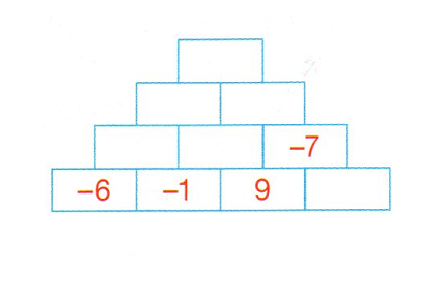
\includegraphics[scale=1]{pyramide.eps} \\
\end{center}

\newpage

\exo{2} Calculer astucieusement :		

\bmul{2} 
\begin{flushleft}
$A = (+ 13,5) + (- 8,1) + (- 6,9) + (+ 5,5)$\\
\reponse[5]
\end{flushleft}
 
 \columnbreak
 
\begin{flushleft}
$B = (- 10,9) + (+ 6) - (+ 8,7) + (+ 5,3) + (- 12) - (- 5,3)$\\
\reponse[5]
\end{flushleft}

\emul




\end{document}
